\subsubsection{SLATE}\label{subsubsect:slate}


\paragraph{Overview}

The objective of the Software for Linear Algebra Targeting Exascale 
(SLATE) project is to provide fundamental dense linear algebra capabilities
to the US Department of Energy (DOE) and to the high-performance 
computing (HPC) community at large.
To this end, SLATE will provide basic dense matrix operations (e.g., matrix multiplication,
rank-k update, triangular solve),
linear systems solvers, least square solvers, singular value
and eigenvalue solvers.

The ultimate objective of SLATE is to replace the
venerable Scalable Linear Algebra PACKage (ScaLAPACK) library, 
which has become the industry standard
for dense linear algebra operations in distributed memory environments.
However, after two decades of operation, ScaLAPACK is past the end of its lifecycle
and overdue for a replacement, as it can hardly be retrofitted
to support hardware accelerators, which are an integral part of today's HPC
hardware infrastructure.

Primarily, SLATE aims to extract the full performance potential and maximum 
scalability from modern, many-node HPC machines with large numbers of cores
and multiple hardware accelerators per node.
For typical dense linear algebra workloads, this means getting close to 90\% 
of the theoretical peak performance and scaling to the full size of the machine
(i.e., thousands to tens of thousands of nodes).
This is to be accomplished in a portable manner by relying on standards like 
MPI and OpenMP.

SLATE functionalities will first be delivered to the ECP applications
that most urgently require SLATE capabilities 
(e.g., EXAALT, NWChem, QMPACK, GAMESS, and CANDLE)
and to other software libraries 
that rely on underlying dense linear algebra services (e.g., FBSS).
SLATE will also fill the void left by ScaLAPACK's inability to utilize
hardware accelerators, and it will ease the difficulties associated with ScaLAPACK's
legacy matrix layout and Fortran API.
Figure~\ref{fig:slate-architecture} shows SLATE within 
the ECP software stack.

\begin{figure}[htb]
    \centering
    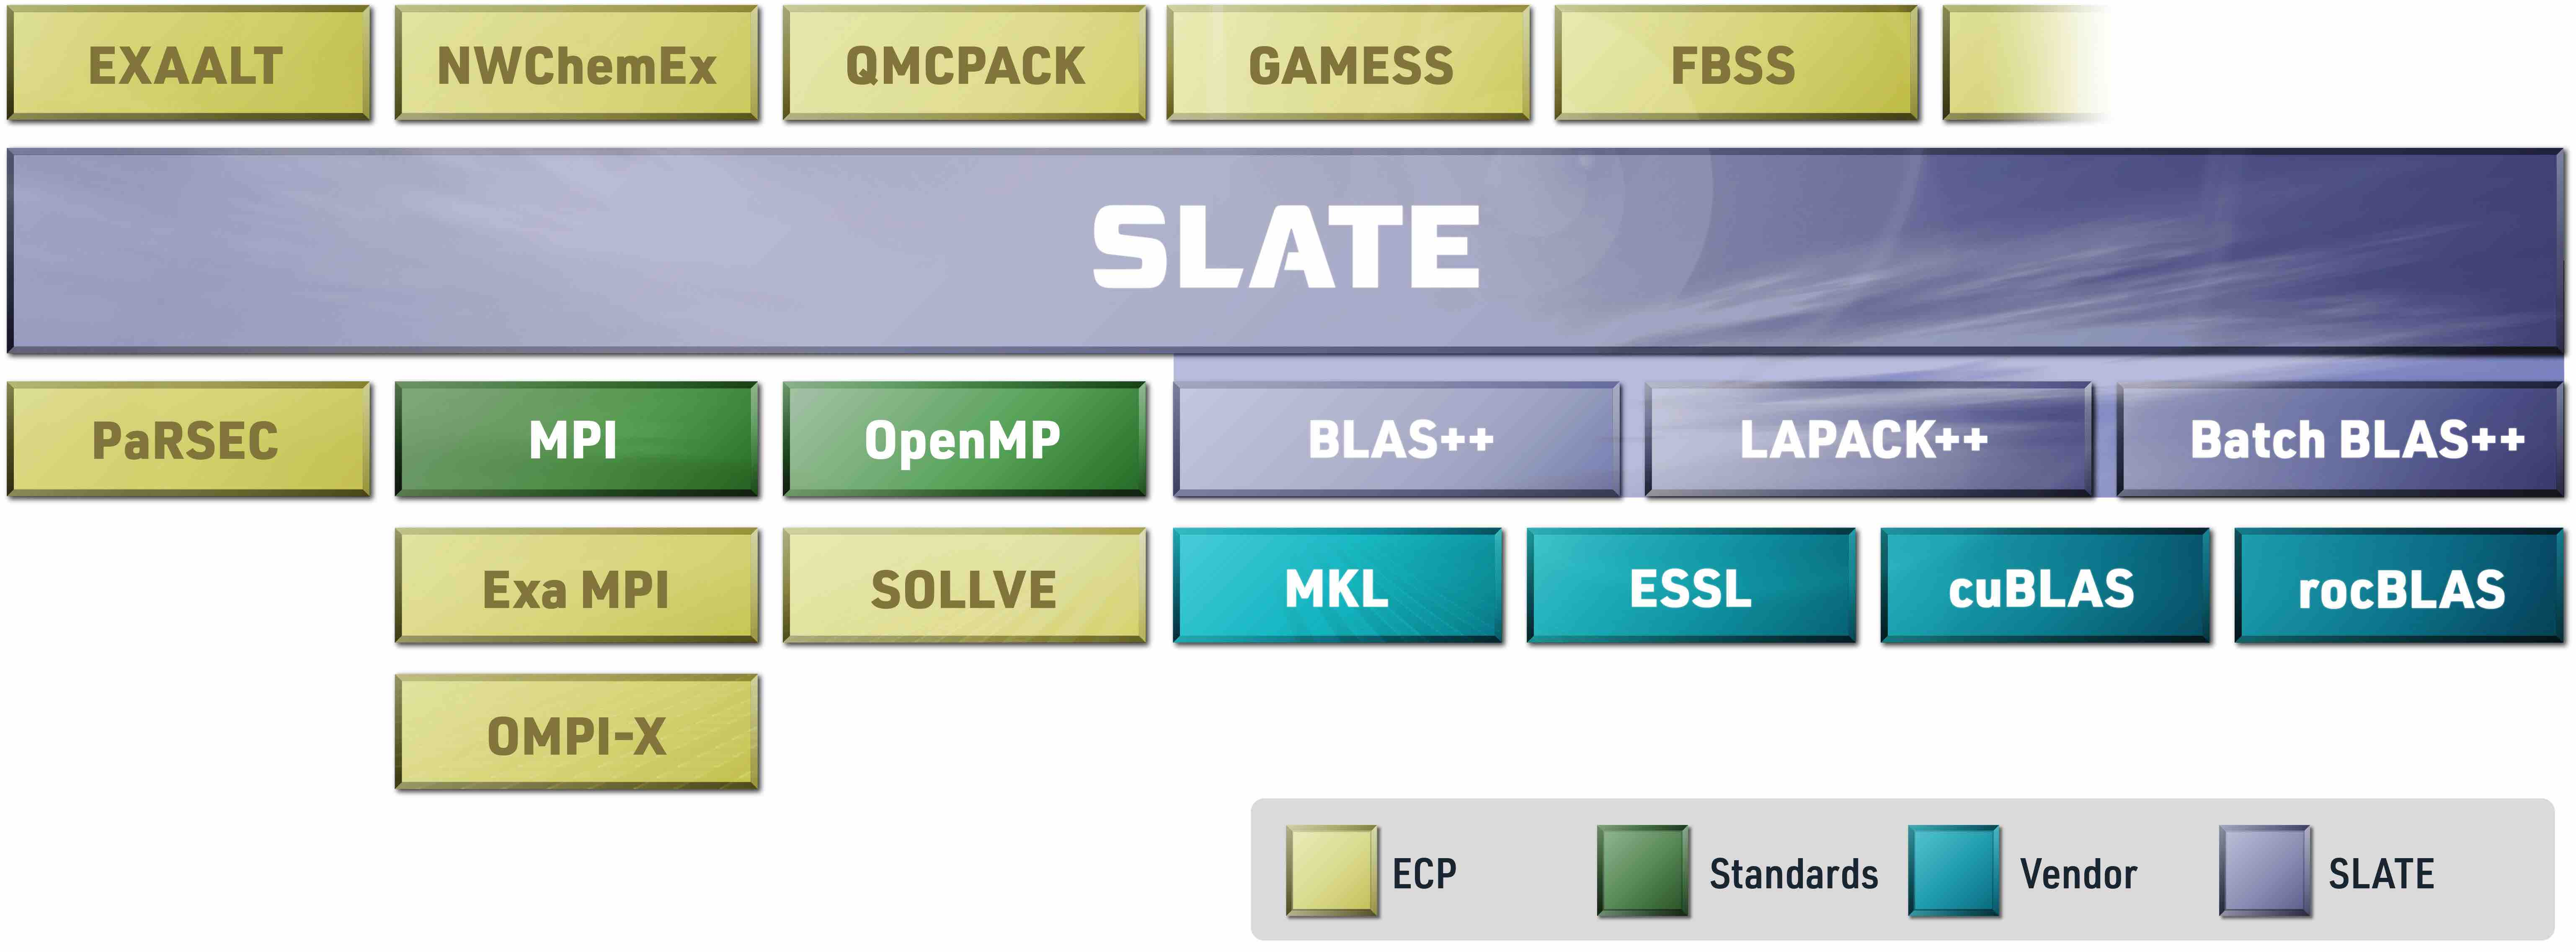
\includegraphics[width=0.6\textwidth]{projects/2.3.3-MathLibs/2.3.3.09-SLATE/SLATE-architecture.jpg}
    \caption{\label{fig:slate-architecture}
    SLATE in the ECP software stack.}
\end{figure}

\paragraph{Key  Challenges}

\begin{enumerate}
\item
\textbf{Designing from the ground up:}
The SLATE project's primary challenge stems from the need to design the package
from the ground up, as no existing software package offered
a viable path forward for efficient support of hardware accelerators in
a distributed-memory environment.
\item
\textbf{Aiming at a hard hardware target:}
SLATE's acceleration capabilities are being developed in an unforgiving
hardware environment, where the computing power of the GPUs exceeds the computing
power of the CPUs, as well as the communication capabilities of the network,
by orders of magnitude.
\item
\textbf{Using cutting-edge software technologies:}
Finally, SLATE is being designed using cutting-edge software technologies,
including modern features of the C++
language, as well as fairly recent extensions of the OpenMP standard
and the MPI standard.
\end{enumerate}

\paragraph{Solution Strategy}

\begin{enumerate}
\item
\textbf{Deliberate design phase:}
The need for building SLATE from scratch was a 
primary focus of SLATE's architecture and design in the initial project
milestones. First, we conducted a careful analysis of all the relevant 
technologies---existing and emerging~\cite{abdelfattah2017roadmap}.
% \footnote{\url{http://www.icl.utk.edu/publications/swan-001}}
Then we designed the initial architecture~\cite{kurzak2017designing}.
%\footnote{\url{http://www.icl.utk.edu/publications/swan-003}}
Going forward, the development process is based on alternating
feature development with refactoring and redesign
of the underlying infrastructure.
\item
\textbf{Accelerator-centric focus:}
Hardware accelerators (e.g., graphic processing units [GPUs]), are treated
as first-class citizens in SLATE, and accelerated performance is the
primary focus of the performance engineering efforts.
Device performance relies on highly optimized routines in vendor libraries,
mostly the batch matrix multiply routine (i.e., batch gemm).
Care is also taken to hide accelerator communication in addition
to hiding message passing communication.
To address the network deficiencies in the long term, the team is investigating
cutting-edge algorithmic solutions like
communication-avoiding algorithms
\cite{ballard2011minimizing}
and randomization algorithms
\cite{mahoney2011randomized}.
\item
\textbf{Community engagement:}
The SLATE team maintains regular contact with the OpenMP community,
the ECP SOLLVE project, and the broader OpenMP community
(joining the OpenMP ARB). The team also engages vendors and has
contacts at Intel, NVIDIA, and AMD. The SLATE team is co-located with the ECP OMPI-X 
project and has a direct line of communication with the MPI community.
\end{enumerate}

\paragraph{Recent Progress}

The most recent development in SLATE is the implementation of all
level-3 PBLAS routines, covering all four precisions,
single real (S), single complex (C), double real (D), double complex (Z),
and all combinations of input parameters, \texttt{side}, \texttt{uplo}, and \texttt{trans}.
SLATE's accelerated runs deliver up to a $20\times$ performance improvement
over ScaLAPACK multi-core runs on the SummitDev machine at the Oak Ridge Leadership
Computing Facility
\footnote{\url{https://www.olcf.ornl.gov/kb_articles/summitdev-quickstart/}}
(Figure~\ref{fig:slate-dgemm}).
A more exhaustive performance analysis is available in
``SLATE Working Note 5: Parallel BLAS Performance Report,''~\cite{kurzak2018parallel}.
%\footnote{\url{http://www.icl.utk.edu/publications/swan-005}}

\begin{figure}[htb]
    \centering
    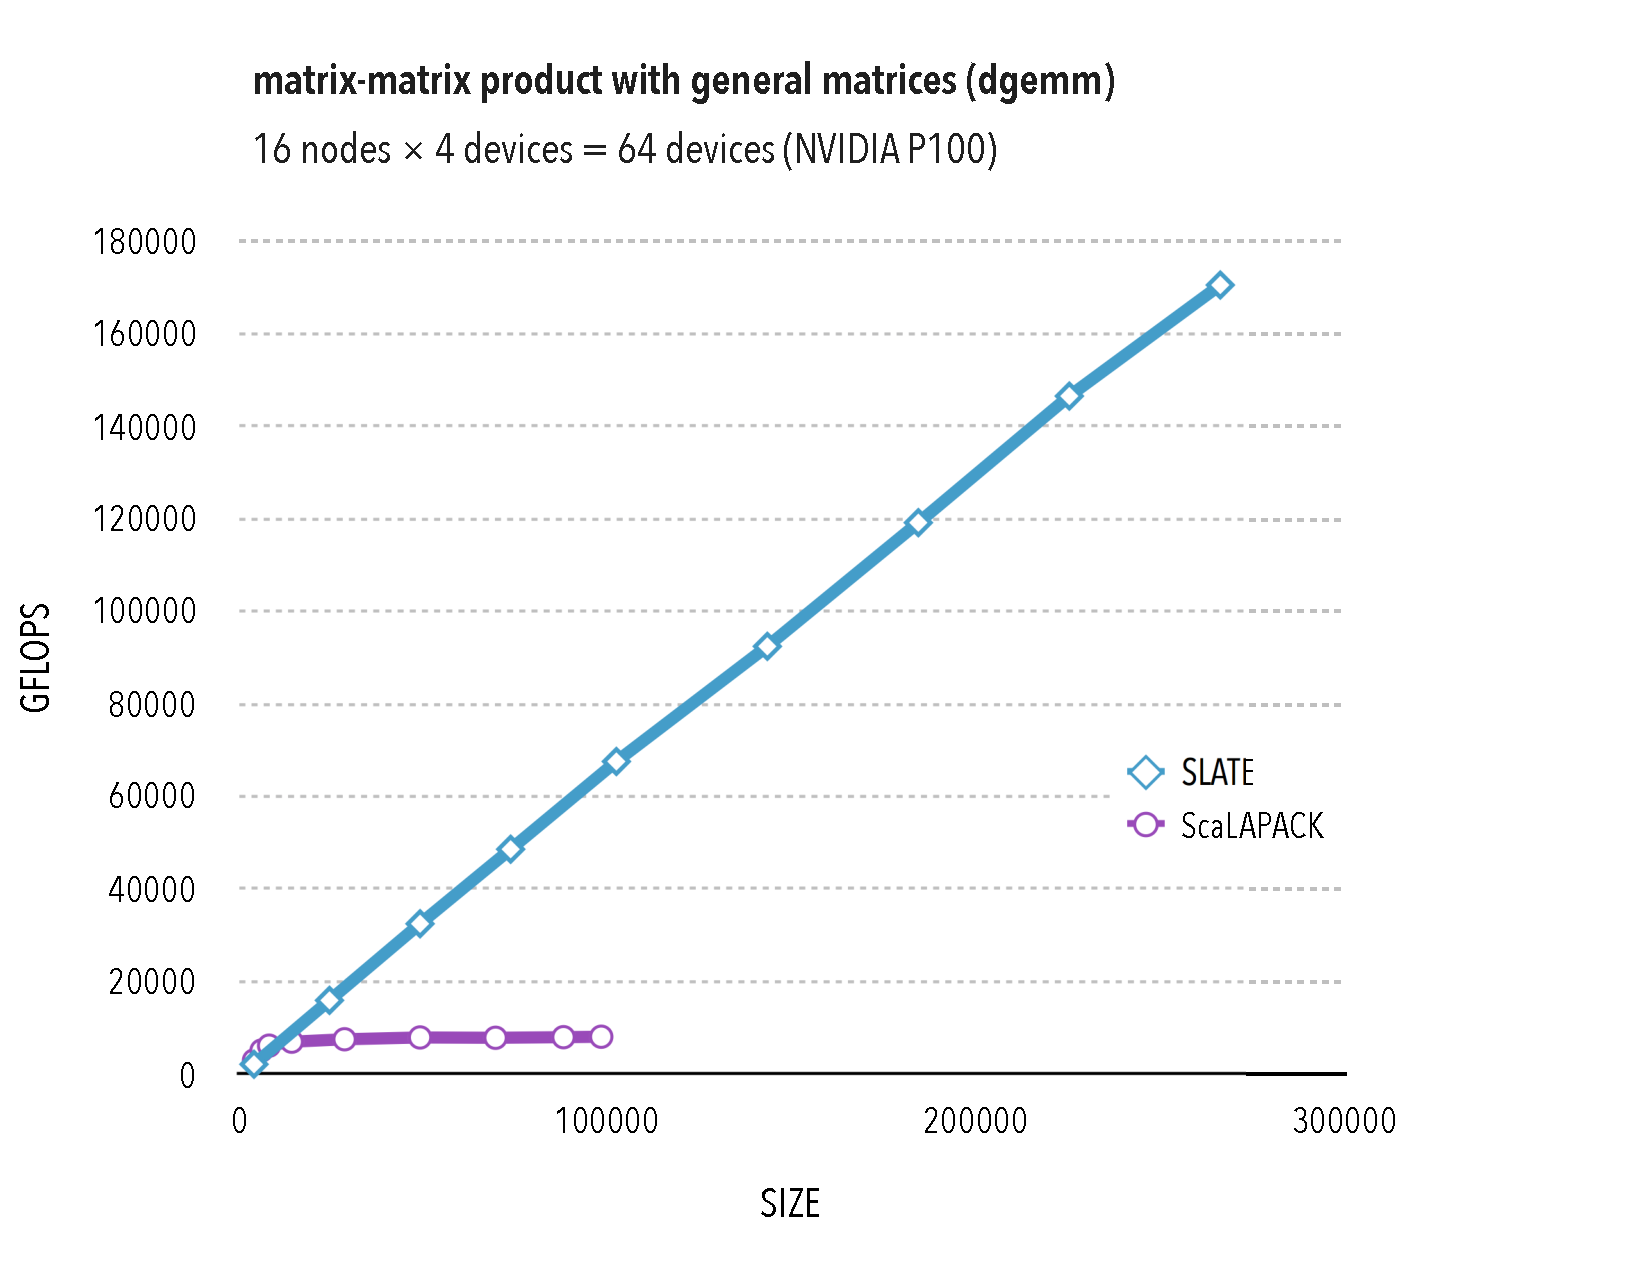
\includegraphics[width=0.55\textwidth]{projects/2.3.3-MathLibs/2.3.3.09-SLATE/SLATE-dgemm.pdf}
    \caption{\label{fig:slate-dgemm}
    Accelerated performance using SLATE compared to multi-core performance using ScaLAPACK.}
\end{figure}

\paragraph{Next Steps}

\begin{enumerate}
\item
\textbf{Matrix norms:}
We plan to implement matrix norms by the end of June 2018.
This includes routines for computing the one norm, max norm, infinity norm,
and a specialized routine for computing a column-wise norm, which is required
for mixed-precision linear solvers based on iterative-refinement.
\item
\textbf{Linear solvers:}
We plan to implement linear solvers by the end of September 2018.
This includes an LL$^T$ factorization, an LU factorization, an LDL$^T$ factorization,
and the corresponding forward/backward substitution routines.
\item
\textbf{Least squares solvers:}
We will implement least squares solvers by the end of December 2018,
including the QR and LQ factorizations and the routines for the
generation and application of the Q matrices.
\end{enumerate}
All four standard ScaLAPACK precisions will be covered,
and all routines will support hardware acceleration.
